% acmsmall-sample.tex, dated 15th July 2010
% This is a sample file for ACM small trim journals
%
% Compilation using 'acmsmall.cls' - version 1.1, Aptara Inc.
% (c) 2010 Association for Computing Machinery (ACM)
%
% Questions/Suggestions/Feedback should be addressed to => "acmtexsupport@aptaracorp.com".
% Users can also go through the FAQs available on the journal's submission webpage.
%
% Steps to compile: latex, bibtex, latex latex
%
% For tracking purposes => this is v1.1 - July 2010

\documentclass[prodmode,acmtaco]{acmsmall}

% Package to generate and customize Algorithm as per ACM style
\usepackage[ruled]{algorithm2e}
\renewcommand{\algorithmcfname}{ALGORITHM}
\SetAlFnt{\small}
\SetAlCapFnt{\small}
\SetAlCapNameFnt{\small}
\SetAlCapHSkip{0pt}
\IncMargin{-\parindent}

\usepackage{graphicx,url}
\usepackage{listings}
\usepackage{subfigure}
\usepackage{multirow}
\usepackage{pictexwd}
\usepackage[absolute]{textpos}
\usepackage[english]{babel}
\usepackage{footnote}
\usepackage{listings}
\lstset{keywordstyle=\bfseries, flexiblecolumns=true}                           
\lstloadlanguages{[ANSI]C++}
\lstdefinestyle{prg} {basicstyle=\small, lineskip=-0.2ex, showspaces=false,breaklines=true,showstringspaces=false,numbers=left,numbersep=-7pt,frame=single,stepnumber=1}

\newcommand{\prg}[3][ht!]{
  \begin{figure}[#1]
      \lstinputlisting[language=C++,style=prg,xrightmargin=.2\textwidth,xleftmargin=.2\textwidth]{fig/#2.cc}
    \caption{#3\label{prg:#2}}
  \end{figure}
}

\newcommand{\prgFull}[3][ht!]{
  \begin{figure}[#1]
      \lstinputlisting[language=C++,style=prg]{fig/#2.cc}
    \caption{#3\label{prg:#2}}
  \end{figure}
}

\newcommand{\fig}[4][ht!]{
  \begin{figure}[#1]
    {\centering{\includegraphics[#4]{fig/#2}}\par}
    \caption{#3}
    \label{fig:#2}
  \end{figure}
}


\newcommand{\Fig}[4][hp]{
  \begin{figure*}[#1]
    {\centering{\includegraphics[#4]{fig/#2}}\par}
    \caption{#3}
    \label{fig:#2}
  \end{figure*}
}

% Metadata Information
\acmVolume{1}
\acmNumber{1}
\acmArticle{1}
\acmYear{2012}
\acmMonth{1}

% Document starts
\begin{document}

% Page heads
\markboth{G. Gracioli and A. A. Fr\"{o}hlich.}{Monitoring Shared Memory Invalidations in Embedded Multicore Software through HPCs}

% Title portion
\title{Monitoring Shared Memory Invalidations in Embedded Multicore Software through HPCs}
\author{GIOVANI GRACIOLI and ANT\^{O}NIO AUGUSTO FR\"{O}HLICH
\affil{Federal University of Santa Catarina}}

\begin{abstract}
%Multicore processors are a reality in embedded real-time systems. Mainly due to the unpredictability on their memory hierarchy, however, it is hard to bound worst-case execution scenarios, which is essential in real-time applications. In these processors, the coherence between the memory hierarchy is kept by a coherence protocol, typically based on bus snooping. Excessive bus snooping, caused by a frequent rate of data sharing (e.g., cache line invalidations), can violate real-time guarantees. Thus, it is important to monitor and detect when excessive cache line invalidations occurs. Hardware Performance Counters (HPCs) are an alternative to this purpose. In this paper, we present a lightweight HPCs interface for embedded real-time systems and by using a benchmark, we analyze the relation between the software and the cache coherence protocol in a current multicore processor. Results have shown that HPCs provide a correct view of the application behavior and can be used at run time to detect when excessive invalidations happens.
The use of multicore processors in embedded real-time systems is not straightforward due to their unpredictability in bounding worst-case execution scenarios due to coherence through memory hierarchy (bus snooping). Hardware Performance Counters (HPCs) are an alternative to monitor when excessive memory invalidations occurs and thus avoiding deadline misses. In this paper, we present a HPC interface for embedded systems. By using a benchmark, we analyze the relation between the software and the cache coherence protocol in a multicore processor. Results have shown that HPCs provide a correct view of the application behavior and can be used to help OS decisions.
\end{abstract}

\category{D.4.1}{Operating Systems}{Process Management -- Multiprocessing/multiprogramming/multitasking, scheduling, threads}
\category{D.4.7}{Operating Systems}{Organization and Design -- Real-time systems and embedded systems}
\category{D.4.8}{Operating Systems}{Performance -- Measurements, monitors}
\category{C.1.2}{Processor Architectures}{Multiple Data Stream Architectures (Multiprocessors) -- Multiple-instruction-stream, multiple-data-stream processors (MIMD)}

\terms{Design, Experimentation, Measurement, Performance}

\keywords{Cache coherence, multicore architectures, memory invalidation, hardware performance counters}

\acmformat{Gracioli, G. and Fr\"{o}hlich A. A. 2011. Monitoring Shared Memory Invalidations in Embedded Multicore Software through Hardware Performance Counters.}

\begin{bottomstuff}
This work was supported by the Coordination for Improvement of Higher Level Personnel (CAPES) grant, project RH-TVD 006/2008.

Authors' address: Software/Hardware Integration Lab, Federal University of Santa Catarina, 88040-900, Florian\'{o}polis, Santa Catarina, Brazil.
\end{bottomstuff}

\maketitle

\section{Introduction}

Multicore processors are being increasingly used in embedded real-time systems due to the evolution and integration of features and consequently the need for more processing power. In automotive environment, for instance, new safety functionalities like ``automatic emergency breaking" and ``night view assist" should read and fusion data from sensors, process the video, and give warnings when an obstacle is detected on the road under real-time constraints~\cite{Mohan2011}. In addition, adding more functionalities to the system costs in terms of power consumption, heat dissipation, and space (e.g. cables)~\cite{Cullmann10a}. Thus, multicore processors become an alternative to decrease these costs and to integrate features in a single processing unit, instead of several ECUs spread over the vehicle.

However, real-time guarantees in multicore architectures are difficult to predict mainly when concurrent threads share different physical resources, such as cache memory, buses, and peripherals. In this context, the memory hierarchy is an important bottleneck for performance and timing predictability~\cite{Marwedel2005,Muralidhara:2010,Zhuravlev:2010}. Usually, a Level-1 cache is private to a core, while a Level-2 and/or a Level-3 cache is shared among cores. Each core has its own data and uses its private cache for speeding up the processing. When cores share data, each copy of data is placed in the core's private cache and a cache-coherence protocol (e.g., MESI~\cite{Patterson:06}, MOESI~\cite{amd64}, or MESIF~\cite{intel}) is responsible for keeping the consistency between each copy through bus snooping.

When a core writes into a data that other cores have cached, the cache-coherence protocol invalidates all copies, causing an implicit delay in the application's execution time. Moreover, when a core reads a shared data that was written by another core, the cache-coherence protocol does not return the data until it finds the cache that has the data, annotate that cache line to indicate that there is shared data, and recover the data to the reading core. These operations are automatically performed by the hardware and take hundreds of cycles (about the same time as accessing the off-chip RAM), also increasing the application's execution time. Two kinds of scaling problem occur due to shared memory contention~\cite{BoydWickizer:10}: access serialization to the same cache line done by the cache coherence protocol, which prevents parallel speedup, and saturation into the inter-core interconnection, also preventing parallel processing gains.

Hence, it is important to correctly monitor when excessive shared memory invalidations occurs. In this context, Hardware Performance Counters (HPCs) are a good alternative. HPCs are special registers available in the most modern microprocessors through the hardware Performance Monitoring Unit (PMU). HPCs offer support to counting and/or sampling several micro-architectural events, such as cache misses and retired instructions, at execution time~\cite{Sprunt:02,Azimi:2005}. In multicore processors, for instance, it is possible to count the numbers of snoop requests, last-level cache misses, and evicted cache lines. The events measured by HPCs can provide to the operating system a global and accurate view of the application status. Based on this, the OS can take a decision to improve the application's performance~\cite{Zhuravlev:2010,Azimi:2009}.

In this paper we make the following contributions:

\begin{itemize}
 \item We design a lightweight software interface for a family of PMUs based on concepts from the Application-Driven Embedded System Design (ADESD)~\cite{Froehlich:2001}. The interface is simple and specifically designed to the embedded real-time system domain.
 \item We demonstrate the relation between the cache snooping protocol and the application by measuring hardware events on a real multicore processor through the designed interface. 
 \item We provide an analysis considering the number of cache lines snooped in one core by another one. Due to the high frequency of snoops the application's execution time is affected and consequently deadlines can be lost. 
%In addition, we show how to integrate the created interface with the OS scheduler in order to make smarter scheduling decision.
\end{itemize} 

%\fig{coop_threads}{An example of pipeline application composed by threads sharing data.}{scale=.6}

The remainder of this paper is organized as follows. Section~\ref{sec:back} gives an overview about cache coherence on multicore processors. Section~\ref{sec:interface} presents a lightweight software interface for hardware PMUs. Section~\ref{sec:analysis} provides an analysis about HPCs in the context of memory coherence on multicore processors. Section~\ref{sec:related} discusses the related works. Finally, Section~\ref{sec:conc} concludes the paper.

\section{Cache Coherence on Multicore Processors}
\label{sec:back}

The coherence among the cores' cache is carried out by a cache coherence protocol implemented as a finite state machine in the hardware cache controller located at each core. This protocol is usually an invalidation protocol -- cache controllers snoop every transaction on the shared bus and take an action to ensure coherence. This action depends on the cache coherence protocol and the state of the cache line being requested or modified. MESI, MOESI, and MESIF are examples of cache coherence protocols widely used in today's multicore processors. Our focus on this paper is the MESI protocol. The MESI protocol is the most common cache-coherence protocol which supports write-back cache and it is traditionally used in Uniform Memory Access (UMA) multicore architectures~\cite{Patterson:06}. An example of a processor that uses this architecture is the dual-core Freescale MPC8641D, which is utilized by the avionics industry~\cite{Cullmann10a}.

In MESI, each cache line can be in one of the four states: 

\begin{itemize}
	\item \textbf{Modified (M):} the cache line is not shared and its data is dirty.
	\item \textbf{Exclusive (E):} the cache line is not shared and it is clean.
	\item \textbf{Shared (S):} the cache line is shared by other caches and it is clean.
	\item \textbf{Invalid (I):} the cache line does not hold a valid copy of data. The valid data can be in the main memory or in another processor cache.
\end{itemize}

Figure~\ref{fig:mesi_state_diagram} shows a state machine for the MESI protocol. There are two kinds of state transitions, those initiated by a processor and those due to the events snooped on the bus. A processor read causes a bus read on a read miss. As a result, the cache line state is changed to S (valid copy in another cache -- RMS) or E state (no cache has the required address -- RME). No state transition is performed on a read hit. In a processor write, a S cache line is changed to the M state (WH) and causes a bus transaction to invalidate other copies (SHW). If the cache line written is in the E or M state, there is a transition to the M state (WH) and no bus transaction is performed.

\fig{mesi_state_diagram}{MESI protocol state machine.}{scale=.3}

When a core receives a snoop read request for a cache line in E state, it demotes this cache line from E to S state, since another cache has a copy of the data. When the cache line is in M state, the cache line should be written-back to the memory and the state should be changed to S. In response to a processor write, the bus snoop protocol invalidates or flushes the cache line. 

%\subsection{Hardware Performance Counters}

%HPCs are special registers available in the most modern microprocessors through the hardware Performance Monitoring Unit (PMU). HPCs offer support to counting and/or sampling several micro-architectural events, such as cache misses and retired instructions, at execution time~\cite{Sprunt:02}. However, they are difficult to use due to the limited hardware resources (for example Intel Nehalem supports event counting with seven event counters and AMD Opteron provides four HPCs to measure hardware events) and complex interface (e.g. low-level and specific to micro-architecture implementation)~\cite{Azimi:2005}.

%Nevertheless, it is possible to use multiplexing techniques in order to overcome the limitation in the number of HPCs~\cite{May:01, Sprunt:02} or specific libraries that make the use of HPCs easier~\cite{Dongarra:2003}, yet adding a low overhead to the application. HPCs can be used together with OS techniques, such as scheduling and memory management, to monitor and identify performance bottlenecks in order to perform dynamic optimizations~\cite{Azimi:2009}. In multicore systems, for instance, it is possible to count the numbers of snoop requests, last-level cache misses, and evicted cache lines. 

%Intel PMU family overview.

\section{Hardware Mediator Interface for PMUs}
\label{sec:interface}

Designing and implementing software for embedded systems is not a straightforward task. Embedded systems usually have a wide variety of platforms and the software must be reused in as many projects as possible. Another characteristic is the communication between software and hardware. Traditional Hardware Abstraction Layers (HALs), initially designed to the non-embedded world, can use a substantial amount of extra code which makes the communication between software and hardware devices slower. In summary, the software layer responsible for managing hardware devices should be simple, fast, portable, and have a reduced code size~\cite{Marcondes:2006}.

In this context, the Application-Driven Embedded System Design (ADESD) ~\cite{Froehlich:2001}, a methodology to design a complete embedded system from the source code to hardware components, has the hardware mediator concept~\cite{Polpeta2004}. Hardware mediators are functionally equivalent to device drivers in \textsc{Unix}, but do not build a traditional HAL. Instead, they sustain the interface contract between abstractions and hardware components by means of static metaprogramming techniques that ``dilute'' mediator code into abstractions at compile-time (no calls, no layers, no messages; mostly embedded assembly). 

By using the hardware mediator concept, we have designed a hardware mediator interface for the Intel PMU family. Figure~\ref{fig:pmu_class_diagram} shows the UML class diagram of the interface. The Intel processors, depending on the microarchitecture (e.g., Nehalem, Core, Atom, etc), have different PMU versions. Each version provides different features and variable number of HPCs. For example, the PMU version 2 has two performance counters that can be configured with general events and three fixed performance counters that count specific events, while the PMU version 3 extends the version 2 and provides support for simultaneous multi-threading, up to 8 general-purpose performance counters, and precise event based sampling~\cite{intelsys}. Yet, pre-defined architectural events, such as unhalted core cycles, last-level cache misses, and branch instruction retired, are shared by all the three versions.

\fig{pmu_class_diagram}{UML class diagram for the PMU hardware mediators interface.}{scale=.3}

Configuring an event involves programming performance event select registers (IA32\_PERFEVTSELx) corresponding to a specific physical performance counter (IA32\_PMCx). In order to select an event, the PERFEVTSELx register must be written with the selected event, unit, and several control masks. The unit mask qualifies the condition that the selected event is detected. For example, to configure the PMC0 to count the number of snoop responses to bus transactions, the PERFEVTSEL0 must be written with the EXT\_SNOOP event mask (0x77) and two unit masks that define the conditions when the event should be counted. 

The designed PMU hardware mediator family represents the described Intel PMU organization. A base class IA32\_PMU implements the Intel PMU version 1 and common services for both version 2 and 3, including the pre-defined architectural events. Also, this class declares memory mapped registers and PMCs. The IA32\_PMU\_Version2 and IA32\_PMU\_Version3 extends the base class and implement specific services only available on that version. Finally, available hardware events are listed by specific microarchitecture classes. For instance, Intel\_Core\_Micro\_PMU and Intel\_Nehalem\_PMU list all available events masks for the Intel Core Microarchitecure and Intel Nehalem microarchitectures, respectively.

The hardware mediator interface could be used by a platform-independent component. This component is the one responsible for implementing ``intelligent'' logic by using the mediators. For instance, event ratios such as Cycles per Retired Instruction (CPI), parallelization ratio, modified data sharing ratio, and bus utilization ratio, combine two or more hardware events in order to provide useful insight into the application performance issues~\cite{intelperf}. Moreover, a platform-independent component could also multiplex the hardware counters in order to overcome the limitation on the number of hardware counters. Multiplexing techniques divide the usage of counters over the time, providing to users a view that there exists more hardware counters than processors really support~\cite{Dongarra:2003}. 

As an example to demonstrate the performance of the API, we used the PMC0 to count the EXT\_SNOOP event. The method for configuring the counter occupied 32 bytes and 11 instructions and the method for reading the counter occupied 100 bytes and 40 instructions (Section~\ref{sec:analysis} provides a code example of how these methods were implemented). Other APIs designed to general-purpose computing, such as PAPI~\cite{papi}, require the initialization and creation of lists or event sets that decrease the performance. Moreover, these APIs provide several functionalities that cannot be of interesting of an embedded real-time application. Thus, an interface specific tailored for the application's needs can provide a better performance. It is not our objective, however, to compare the approaches because they are from different domains. The proposed interface could also be easily implemented to represent other PMU families, such those from the PowerPC and ARM processors.

\section{Analysis of HPCs and the cache coherence protocol}
\label{sec:analysis}

In order to analyze the HPCs when there is excessive memory invalidations due to the cache coherence protocol, we have designed a benchmark to generate invalidations composed of two versions of an application and a best-case application for comparing purposes (Figure~\ref{fig:apps}):

\begin{itemize}
 \item \textbf{Sequential}: in this version, two functions are executed in a sequential order. There are no memory conflicts (Figure~\ref{fig:sequential}). The objective of this version is to simulate an algorithm implemented in hardware, that is, it does not face the shared memory invalidation problem.

 \item \textbf{Parallel}: two threads run at the same time and share data (Figure~\ref{fig:parallel}). The objective of this version is to evaluate the performance of the previous version when it is implemented in a multicore architecture. Both functions (1 and 2) from sequential and parallel versions have the same operations and memory accesses (see Figure~\ref{prg:app_loop}). Common sense dictates that this version should run about two times faster than the sequential one. Consequently, if the sequential version is schedulable (proved by a schedulability analysis), the parallel version should be schedulable as well. We do not use any kind of synchronization (i.e., semaphores, mutexes, or condition variables) to ensure data consistency because we are only interested in measuring the shared data contention overhead.

 \item \textbf{Best-case application}: two threads run at the same time, but do not share data (Figure~\ref{fig:best-case}). This application should run about 2 times faster than the sequential one in a multicore processor. The objective is to have a best-case scenario comparable to the other two versions.
\end{itemize}

\begin{figure}[ht]
\centering
\begin{tabular}{ccc}
	\subfigure[] {
	\fbox{
	\includegraphics[scale=.6]{fig/seq_app}
	\label{fig:sequential}}} &
	\subfigure[] {
	\fbox{
	\includegraphics[scale=.6]{fig/par_app}
	\label{fig:parallel}}} & 
	\subfigure[] {
	\fbox{
	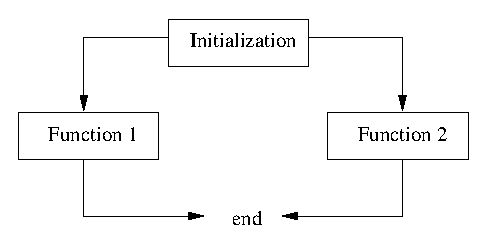
\includegraphics[scale=.6]{fig/best_case_app}
	\label{fig:best-case}}}\\
\end{tabular}
\caption{Benchmark applications: (a) sequential (b) parallel (c) best-case.}
\label{fig:apps}
\end{figure}

All three applications have two two-dimensional arrays of varying size ROWS x COLS and a loop of 10000 repetitions, in which math operations are executed (see Figure~\ref{prg:app_loop}). The shared data in the parallel version is accessed by reading and writing in both arrays and in the same positions, thus we are sure that both threads are accessing the corresponding cache line. At initialization phase, the arrays are started with zero and the threads are created (parallel and best-case applications). The benchmark was implemented as an EPOS\footnote{EPOS is available online at \url{http://epos.lisha.ufsc.br}.} application. EPOS (Embedded Parallel Operating System)~\cite{Froehlich:2001} is a multi-platform, component-based, embedded system framework implemented following the ADESD methodology. It offers support for several architectures and real-time schedulers~\cite{Marcondes2009}, including the CPU\_Affinity multicore scheduler used on the experiments of this paper. Each thread was assigned to a different core (its affinity) and no other thread was executed (3 threads in total, the 2 functions and the main). No thread migrations between cores was performed. All tests were executed in the Intel Core 2 Q9550 processor (Table~\ref{tab:q9550}).

\prg{app_loop}{Part of the source code of sequential and parallel applications.}

\begin{table}[ht!]%
\begin{center}
\tbl{Intel Core 2 Q9550 processor features.\label{tab:q9550}}{%
\begin{tabular}{|c|c|}
\hline
\multicolumn{2}{|c|}{\textbf{Intel Q9550 Features}}\\
\hline
Frequency 			& 2.83 Ghz \\
\hline
Instruction set 	& 64 bits \\
\hline
Physical dies 		& 1\\
\hline
Cores per die 		& 4 (2 dual-core) \\
\hline
Bus speed 			& Front-side bus 1.3 Ghz \\
\hline
L1 private data cache 	& 64 KB 8-way set associative \\
\hline
L2 cache size 		& 12 MB (2x 6 MB) 24-way set associative\\ 
\hline
Cache line size 	& 64 bytes \\
\hline
Memory architecture	& UMA\\
\hline
Coherence protocol 	& MESI \\
\hline
PMU Version 	& 2 \\
\hline
Microarchitecture 	& Intel Core Microarchitecture\\
\hline
\end{tabular}}
\end{center}	
\end{table}

Figure~\ref{fig:avg_execution_time} presents the average execution time (in logarithm scale) for each application version. We ran each application for 10 times and then computed the average execution time. ROWS and COLS for each array were set to 64x64 (32~KB), 128x128 (128~KB), 256x256 (512~KB), 512x512 (2~MB), 1024x1024 (8~MB), 1536x1024 (12~MB), and 1536x1536 (18~MB) that exceeds the L2 cache memory size. The x axis represents the total memory size of both arrays (considering \textit{integer} as 4 bytes) and the y axis the execution time in seconds measured by the EPOS chronometer component~\cite{Froehlich:Timers:2011}. The standard deviation of all versions has presented almost no variation, from 0.01\% to 1\% of the total execution time. We note that, independently of the arrays' size, the parallel version was always slower than the sequential version (up to 1.55 time). As expected, the best-case application was about 2 times faster than the sequential one. This performance degradation is mainly caused by the shared memory invalidations (e.g., bus snooping and MESI cache-coherence protocol), which implies in deadline misses considering the embedded real-time domain if not correctly handled. Lines 9, 10, 13, and 14 in Figure~\ref{prg:app_loop} are responsible for generating bus transactions due to memory coherency that increase the application's execution time.

\fig{avg_execution_time}{Benchmark execution time for each data size.}{scale=.8}

The next step in our evaluation is to use the proposed PMU hardware mediator interface to monitor the hardware events generated by the benchmark. In this context, Figure~\ref{prg:api_example} exemplifies how the interface was used by applications. We implement a component that uses the PMU hardware mediators. This component (\texttt{Perf\_Mon}) provides a high level interface for the applications. For the parallel and best-case versions, we first configured the hardware performance counter to monitor a specific event at the beginning of both functions (\texttt{perf0} and \texttt{perf1}), since they are executed on different cores. For the sequential version, the performance counter is configured before the call to the first function and read after the execution of the function 2, since they are executed in the same core.

\prgFull{api_example}{Example of how the benchmark uses the proposed interface.}

Figure~\ref{prg:perfmon} demonstrates how the \texttt{Perf\_Mon} component uses the PMU hardware mediator. In this example, the method \texttt{cpu\_clk\_unhalted\_bus} configures the performance monitoring counter 0 to monitor the CPU\_CLK\_UNHALTED\_BUS (bus cycles when core is not halted) event. The method \texttt{get\_cpu\_clk\_unhalted\_bus} reads the current value of the counter, that is, the number of bus cycles when the core is not halted.

\prgFull{perfmon}{Example of a component that uses the proposed mediator.}

We then have measured the data bus utilization using the described PMU infrastructure. This metric is given by the CPU\_CLK\_UNHALTED\_BUS event divided by the BUS\_DRDY\_CLOCKS (bus cycles when data is sent on the bus) event. For the sequential and best-case applications, we obtained up to 56\% and 28\% of utilization, while for the parallel application we obtained up to 179\% of data bus utilization when the data size is 12~MB. For all data size less than 12~MB, the maximum data bus utilization was 39\%. When the data size is greater than the cache memory size (18~MB), the data bus utilization decreases to about 3\%. This confirms that frequent share data accesses cause an implicit delay in the application execution time despite the bus utilization.

%\fig{data_bus_utilization}{Data bus utilization for the benchmark. The percentage is given by diving CPU\_UNHALTED\_BUS by BUS\_DRDY\_CLOCKS events.}{scale=.7}

In the next experiment, we have measured the hardware events generated by each application and associated to bus transactions. The analyzed event was the snoop responses to bus transactions (EXT\_SNOOP). Snoop responses can be counted by type as follows~\cite{intelsys}:
%Responses can be counted separately by bus agent (``all agents" mask counts all snoop responses seen on the bus and ``this agent" mask counts snoop responses from this processor to bus transaction sent by this processor). Furthermore, 

\begin{itemize}
	\item \textbf{CLEAN:} this event occurs when the responder's cache does not have the address.
	\item \textbf{HITM:} this event occurs when the snooped address at the responder's cache is in the Modified state.
	\item \textbf{HIT:} this event occurs when the snooped address at the responder's cache is in the Shared or Exclusive state.
\end{itemize}

Additionally, these three types can be combined together. For example, it is possible to combine HIT and HITM to obtain all snoop responses for cache lines that were in the Modified, Shared, or Exclusive states. In our tests, we configured the PMC0 to count snoop responses from this processor to bus transactions sent by this processor (THIS\_AGENT mask). We also vary the type (CLEAN, HIT, and HITM) being counted. Each application version was executed 10 times for each PMC configuration and the average value was used to plot the graphs (more than 1000 executions on a real hardware).

Figure~\ref{fig:HPC_eval} shows the measured values and their standard deviation in logarithm scale. An expected behavior for all cases can be observed: the parallel version always generated more bus responses than the sequential and best-case applications. The explanation for bus responses in sequential and best-case version is the natural implementation of a multicore OS kernel and false sharing. Variables are shared by EPOS to guarantee mutual exclusion for some OS areas (e.g., spinlocks).

\begin{figure*}[htb]
\centering
\begin{tabular}{cc}
	\subfigure[] {
	\includegraphics[scale=.68]{fig/bus_resp_clean}
	\label{fig:bus_clean}} &
	\subfigure[] {
	\includegraphics[scale=.68]{fig/bus_resp_hit}
	\label{fig:bus_hit}
	}\\
	\subfigure[] {
	\includegraphics[scale=.68]{fig/bus_resp_hitm}
	\label{fig:bus_hitm}} &
	\subfigure[] {
	\includegraphics[scale=.68]{fig/bus_resp_clean_hitm}
	\label{fig:bus_clean_hitm}
	}\\
	\subfigure[] {
	\includegraphics[scale=.68]{fig/bus_resp_clean_hit}
	\label{fig:bus_clean_hit}} &
	\subfigure[] {
	\includegraphics[scale=.68]{fig/bus_resp_hit_hitm}
	\label{fig:bus_hit_hitm}
	}\\
\end{tabular}
\caption{Benchmark HPCs evaluation on Intel Core 2 Quad Q9550 processor. (a) bus snoop responses CLEAN; (b) bus snoop responses HIT; (c) bus snoop responses HITM; (d) combining CLEAN and HITM snoop responses events; (e) combining CLEAN and HIT events; and (f) combining HIT and HITM events.}
\label{fig:HPC_eval}
\end{figure*}
 
In Figures~\ref{fig:bus_clean},~\ref{fig:bus_clean_hitm}, and~\ref{fig:bus_clean_hit}, we can note that the sequential and best-case versions have an exponential behavior in the number of bus responses. When the data size is greater than the L2 cache memory size, all the three applications have almost the same number of bus responses. There are more conflicts for the same cache line in a core -- the L2 cache is full and cache lines are evicted whenever new addresses are read. Consequently, when a core asks for a cache line, the probability that this cache line no longer be in the another core's cache is higher (more CLEAN responses). In addition, as the number of CLEAN events is greater than HITM and HIT events, the curves in Figures~\ref{fig:bus_clean_hitm}, and~\ref{fig:bus_clean_hit} present similar format. They also presented similar behavior when dividing the snoop requests by the total number of shared memory accesses (lines 9, 10, 13, and 14 in Figure~\ref{prg:app_loop})\footnote{This number can be obtained by the following equation: REP x ROWS x COLS x 4 (2 reads and 2 writes).}. The sequential and best-case applications have obtained from 0.0002\% (32~KB) to 3\% (18~MB), while the parallel version obtained from 0.07\% to 3\%. Due to high degree of concurrence (both threads constantly invalidate the data from each other) we observed more CLEAN snoop responses than HIT and HITM. Note that not every memory access generates a bus response (see Section~\ref{sec:back}).

Figure~\ref{fig:bus_hit} shows the number of snoop responses when the responder's cache line is in either S or E states. There is a considerable increase of responses from 2~MB to 8~MB. The parallel version always generated more HIT responses than the other two versions. The relation between memory accesses and bus responses reached almost 2.5\% for the parallel version and 8~MB of data size. For 12~MB and 18~MB the percentage was 1.4\% and 0.3\%. For all the sequential and best-case applications and data sizes the relation was less than 0.0001\%.

Figure~\ref{fig:bus_hitm} shows the snoop responses when the responder's cache is in the M state. When the data size is greater than the L2 cache size, the number of snoop responses in the parallel version decreases, since there is no enough space in the cache for all data. The sequential and best-case applications present similar behavior. The relation between memory accesses and snoop responses decreases whenever the data size increases. For the sequential and best-case applications, this relation was always less than 0.0001\%. For the parallel version, it started in 0.8\% (32~KB) and ended in 0.006\% (18~MB). 

Finally, Figure~\ref{fig:bus_hit_hitm} presents the combination of HIT and HITM events, that is, the number of snoop responses when the responder's cache line is in either S, E, or M states. The curves in the graph are similar to the Figure~\ref{fig:bus_hitm}. We can conclude from these graphs that there are more cache line invalidations happening than cache line hits because the number of snoop responses CLEAN is greater than snoop responses HIT and HITM. However, the snoop responses CLEAN event is also generated when there is false sharing, which is proved when the data size is greater than the L2 cache memory size. False sharing occurs when threads running on different cores access data that resides in the same cache line, not necessary the same data address but data addresses that are in the same cache line. Hence, the CLEAN event is not a good option for detecting excessive data sharing between threads when the working data size is greater than the cache memory size. HIT and HITM, instead, could be used to give to the operating system a correct view of the software's behavior.

Although these events give an idea regarding the bus activity and the sharing pattern between cores, they do not show the introduced overhead. In order to measure the overhead associated to bus activities, we monitor the following events~\cite{intelsys}:

\begin{itemize}
	\item \textbf{BUS\_DRDY\_CLOCKS}: bus cycles when data is sent on the FSB.
	\item \textbf{BUS\_LOCK\_CLOCKS}: bus cycles when the LOCK signal is asserted on the bus due to a locked memory access.
	\item \textbf{BUS\_HIT\_DRV}: bus cycles when the HIT\# pin is asserted to signal HIT snoop response.
	\item \textbf{BUS\_HITM\_DRV}: bus cycles when the HITM\# pin is asserted to signal HITM snoop response.
	\item \textbf{L2\_ADS}: bus cycles while the L2 address bus is being used for accesses to the L2 cache os bus queue.
	\item \textbf{BUS\_BNR\_DRV}: number of Bus Not Ready (BNR) signals asserted on the bus. This signal is asserted to suspend additional bus requests by other bus agents when the number of data and snoop transactions is close to the maximum that the bus can handle. By multiplying this event by two is possible to obtain its bus cycles.
	\item \textbf{BUS\_DATA\_RCV}: number of bus cycles during which the processor is busy receiving data.
\end{itemize}

All events were configured to count hardware events related to a specific core (THIS\_CORE mask) and originated by a specific physical core (THIS\_AGENT mask). We ran each application version varying the data size for each event 10 times. Then, we computed the average values to plot the graphs.

Figure~\ref{fig:bus_trans_cycles} shows the values for each described event, application version, and data size. The percentage inside the bars means the amount of cycles from that event in the total cycles given by the sum of cycles from all events. The parallel version always presented more bus cycles despite the data size. For sequential and best-case applications, from 32~KB to 12~MB, the L2\_ADS event was responsible for almost all measured bus cycles. Since there is less bus transactions (see Figure~\ref{fig:HPC_eval}), almost all bus cycles is spent accessing the L2 cache memory. For the parallel application, instead, we observe more cycles being spent in the L2\_ADS event due to the bus queue. There are more frequent bus transactions and therefore more time is spent on the bus queue. For sequential and best-case version and 18~MB of data size, we observe that the BUS\_DATA\_RCV event has 41\% and 27\% of total cycles. There are more data being moved to/from the cache memory from/to main memory and this is reflected in this event. For the parallel application, however, this event was not significant only when the data size is 8~MB. We can conclude that the BUS\_DATA\_RCV also reflects bus activities. Data is being exchange between cores due to the cache coherence protocol. The L2\_ADS event vary from 41\% to 76\% of cycles in the parallel version. As there is no access to locked memory, the BUS\_LOCK\_CLOCKS event presented less than 0.01\% of the total bus cycles.

Another interesting fact is found in the BUS\_HIT\_DRV event. We have noticed an increasing of HIT snoop responses from 2~MB to 8~MB in Figure~\ref{fig:bus_hit}. We can also observe this increasing in Figure~\ref{fig:bus_trans_cycles} when the data size is 8~MB. The BUS\_HIT\_DRV is responsible for 24\% of all measured bus cycles. For 12~MB and 18~MB, the BUS\_HIT\_DRV decreases to 8\% and 4\%, which can also be seen in the line of Figure~\ref{fig:bus_hit}. We can note that when the data is 8~MB, the BUS\_BNR\_DRV signal presented 4\% of all bus cycles. There is a relation in the number of HIT and bus not ready events. As the number of HIT increases, the number of bus transactions gets close to the maximum that the bus can handle and consequently there are more signals to suspend additional bus requests.

Finally, BUS\_HITM\_DRV and BUS\_DRDY\_CLOCKS events are more representative for data size from 32~KB to 2~MB. The first one vary from 8\% to 4\%. The second vary from 10\% to 3\%. BUS\_HITM\_DRV presented 2\% in the parallel version and 8~MB and less than 1\% for 12~MB and 18~MB. This is the same behavior found in Figure~\ref{fig:bus_hitm}, which the number of bus snoop responses HITM decreases after 8~MB.

\fig{bus_trans_cycles}{Bus cycles associated to hardware bus events.}{scale=.8}

The next evaluation was performed by using the CMP\_SNOOP hardware event configured in the PMC0. This event counts the number of times the L1 data cache is snooped for a cache line that is needed by other core. These snoops are performed through the L1 data cache store port. Therefore, frequent snoops may conflict with extensive stores to the L1 data cache, which may increase store latency and impact performance~\cite{intelsys}. This snoop request may change the state of a cache line, as discussed in Section~\ref{sec:back}.
%CMP\_SNOOP can be configured to count events initiated by both cores or only by one core. Besides, it supports three types of snoops:

%\begin{itemize} 
%	\item \textbf{Invalidate:} counts snoops started by a cache line write request. The snooped cache that holds this cache line must evict it.
%	\item \textbf{Any:} any kind of snoop.
%	\item \textbf{Share:} counts snoops started by a cache line read request. The snooped cache that holds this cache line must modify its state to Shared.
%\end{itemize}

Figure~\ref{fig:l1_data_cache_snooped} shows the number of hardware events when the L1 data cache is snooped by other core causing an invalidation (e.g., the cache line must be evicted) and initiated by all cores. A cache line is either missing in the L1 data cache of the other core or it is available for reading only and the other core wishes to write the cache line. Basically, the lines 13 and 14 from the parallel source code (Figure~\ref{prg:app_loop}) are responsible for invalidations measured by this event.

\fig{l1_data_cache_snooped}{L1 data cache snooped by other core. HPC configured to count invalidate snoops from both cores.}{scale=.8}

The parallel application has presented from 2 to 3 orders of magnitude more snoops than the sequential and best-case applications. Again, the snooped data from sequential and parallel applications is due to the EPOS shared control variables. When the data size is greater than the L2 cache memory (from 12~MB to 18~MB), the parallel version presents a slightly decreasing in the number of snoops. This is due the fact that there is more data being replaced in both caches (e.g., conflicts in the cache lines), and thus the probably of a data to be in the requested cache line is less. The standard deviation of the best-case application vary from about 10\% for 32~KB, and 128~KB data sizes to 0.05\% for 18~MB. The maximum standard deviation for the sequential and parallel versions was 4.82\% for 2~MB data size and 3.49\% for 62~KB data size, respectively. The total number of L1 data snoops represents from 0.04\% to 1.67\% of all writings done by the code in a core for the parallel version and about 0.0005\% for the sequential and best-case versions. Lines 13 and 14 from Figure~\ref{prg:app_loop} are responsible for generating this event -- reads are not considered because they do not generated invalidation transactions.

We then normalized the average number of L1 data cache snoops in a period of 10~ms given by: $ N = \frac{AVG_s}{AVG_{ex} / 10 ms} $, where $AVG_s$ is the average number of snoops (Figure~\ref{fig:l1_data_cache_snooped}) and $AVG_{ex}$ is the average execution time (Figure~\ref{fig:avg_execution_time}). Figure~\ref{fig:l1_data_cache_snooped_period} shows the normalized values. We can note that there is almost no variation for the sequential and best-case applications, about 60 snoops in a period, while for the parallel application there is up to 100.000 snoops in a period. This graph shows the frequency of cache line invalidations and how the hardware event could be used by an OS. For instance, during a scheduling quantum, this event could be monitored and if it measures more than a threshold value, the scheduler could decide to not schedule a thread, move a thread to another core, or decrease the parallelism.

\fig{l1_data_cache_snooped_period}{L1 data cache snooped by other core in a period of 10~ms.}{scale=.8}

%Morever, this graph leads us to a question: what is the minimal frequency of bus snoops that would not compromise the application's performance, that is, the gain due to parallelism? In this context, we first measured the STORE\_BLOCK\_ORDER event. This event informs the number of processor cycles while a store operation is waiting for a preceding stored cache line to be observed by other cores. When the store requires a bus transaction (hits a cache line in the S state for example), the operation only ends when the snoop response for the bus transaction arrives~\cite{intelsys}. Thus, it is possible to measure the overhead associated to bus transactions. The lines 9, 10, 13 and 14 in the Figure~\ref{prg:app_loop} are the responsible for generating this event. Figure~\ref{fig:store_block_order_overhead} shows the overhead in percentage related to the execution time of the parallel application. Acesso mais frequente a mesma linha de cache quando o tamanho dos dados eh menor?

%\fig{store_block_order_overhead}{Store block order overhead for the parallel application.}{scale=.8}

\section{Related Work}
\label{sec:related}
This section discusses several works related to software support for PMUs (e.g. libraries and interfaces), HPCs as an alternative to easily detect sharing pattern among threads and help scheduling decisions, and multicore real-time schedulers.

\subsection{Software support for PMUs}

The Performance API (PAPI) is the most used open source cross-platform interface for hardware performance counters~\cite{Dongarra:2003,papi}. PAPI consists of a machine-dependent layer, a high level interface that provides access to read, start, and stop counters, and a low-level interface that provides additional features. This low-level interface would be the hardware mediators in our implementation. It is not our target, however, to make a comparison between the two implementations. PAPI supports a wide range of platforms, was designed to general-purpose computing systems, and has been under development for more than 10 years. Instead, our interface is designed to embedded applications, which have their requirements known at design time. Thus, it is possible to generate only the needed code for the application and nothing else.

Linux abstracts the usage of HPCs through a performance counter subsystem. A performance monitoring tool (\emph{perf}) uses this subsystem and allows developers to obtain and analyze the performance of their applications. The tool also supports a command to record data into files which can be later analyzed using a \emph{report} command. However, embedded systems usually do not have a control interface. Other tools such as Intel Vtune~\cite{intelperf} and AMD CodeAnalyst~\cite{codeanalyst} offer a ``friendly'' interface to monitor performance of processors and applications through the use of HPCs.

\subsection{HPCs and OS Scheduling}

Bellosa and Steckermeier were the first to suggest using HPCs to dynamically co-locate threads onto the same processor~\cite{Bellosa:1996}. Weissman uses HPCs to guide thread scheduling in SMPs~\cite{Weissman:1998}. His method is based on a shared state cache model that takes as input the number of cache misses, measured by HPCs during a scheduling quantum, and a graph representing the current shared state dependencies among threads. This graph is induced by users annotations in the source code. The objective is to compute the effects of all threads' working sets in the cache of a processor. Based on the model, two scheduling policies are proposed. However, they do not consider the invalidation effects of data sharing between threads running in different processors.

Tam et al. use HPCs to monitor the addresses of cache lines that are invalidated due to cache-coherence activities and to construct a summary data structure for each thread, which contains the addresses of each thread that are fetching from the cache~\cite{Tam:2007}. Based on the information from this data structure, the scheduler mounts a cluster composed by a set of threads, and allocates a cluster to a specific core. However, this approach is not feasible for UMA processors, since there is no performance gains in allocating a thread to a specific core in terms of memory access time. West et al. propose a technique based on a statistical model to estimate per-thread cache occupancies online through the use of HPCs, but data sharing is not considered by the authors~\cite{West:2010}.

Another work to address shared resource contention via scheduling was proposed by Zhuravlev~\cite{Zhuravlev:2010}. The paper identifies the main problems that can cause contention in shared multicore processors (e.g. memory controller contention, memory bus contention, prefetching hardware, and cache space contention). The authors propose two scheduling algorithms (\textit{Distributed Intensity} - DI, and \textit{Distributed Intensity Online} - DIO). DI uses a threads' memory pattern classification as input, and distributes threads across caches such that the miss rates are distributed as evenly as possible. DIO uses the same idea, but it reads the cache misses online, through HPCs. DIO performed better than the Linux CFS both in terms of average performance as well as execution time stability from different executions~\cite{Zhuravlev:2010}. Calandrino and Anderson use HPCs to count the number of cache misses and estimate the working set size (WSS) of each thread~\cite{Calandrino:2009}. Based on the WSSs, a cache-aware real-time scheduler selects threads to be scheduled in such a way that co-runners threads do not thrash the shared cache memory. 

Several scheduling algorithms have been proposed in order to provide real-time guarantee for multicore applications. Brandenburg and Anderson discuss how the implementation of the ready queue, quantum-driven x event-driven scheduling, and interrupt handling strategies affect a global real-time scheduler~\cite{Anderson2009b}. The results indicate that implementation issues can impact schedulability as much as scheduling-theoretic tradeoffs. Moreover, in their case study, the best performance was achieved by using a fine-grained heap, event-driven scheduling, and dedicated interrupt handling. An empirical comparison of Global-EDF (G-EDF), Partitioned-EDF (P-EDF), and Clustered-EDF (C-EDF) on a 24-core Intel platform, assuming run-time overhead (e.g. release, context switch, and schedule times) and cache-related delay, has concluded that P-EDF outperforms the other evaluated algorithms in hard real-time scenarios~\cite{Brandenburg2010a}. Moreover, the same study suggests the use of ``less global" approaches (P-EDF and C-EDF-L2, which cluster at the cache level 2) in contrast of ``more global" approaches (G-EDF and C-EDF-L3) in hard real-time applications. Another real-time scheduler for multiprocessors is proposed by Cho~\cite{Cho2006}. The authors proposed a new abstraction about task execution behavior on multiprocessors, named the time and local remaining execution-time plane (T-L plane). The entire scheduling over time is the repetition of T-L planes in various sizes. Therefore, a single T-L plane scheduling implies on feasible scheduling over all times. Another scheduling algorithm is presented by Srinivasan and Anderson~\cite{Srinivasan2006}. They show that the PD2 Pfair Algorithm is an optimal rate-based scheduling algorithm, since it correctly schedules any feasible intra-sporadic task system on M processors.

In the context of memory-aware real-time multicore scheduling algorithms, Calandrino and Anderson have proposed a cache-aware scheduling algorithm~\cite{Anderson2006,Calandrino2008}. In their approach, the scheduling process is divided in two phases: (i) all tasks that may induce significant memory-to-L2 traffic are combined into groups off-line; and (ii) at run-time, a scheduling policy that reduces concurrency within groups is used. The paper introduces the concept of \emph{megatask}, which represents a task group and is treated as a single schedulable entity. All cores are symmetric, share a chip-wide L2 cache, and each core supports one hardware thread. Nevertheless, the algorithm fails in measuring the real influence of cache thrashing in an environment with threads sharing memory. $FP_{CA}$ is a cache-aware scheduling algorithm that divides the shared cache space into partitions~\cite{Guan2009}. Tasks are scheduled in a way that at any time, any two running tasks' cache spaces (e.g. a set of partitions) are non-overlapped. A task can execute only if it gets an idle core and enough cache partitions. The authors proposed two schedulability tests, one based on a linear problem (LP) and another one as an over-approximation of the LP test. Tasks are not preemptive and the algorithm is blocking, i.e. it does not schedule lower priority ready jobs to execute in advance of higher priority even though there are enough available resources. $FP_{CA}$ is executed whenever a job finishes or a new job arrives.

In general, few related work consider a multicore system where threads share data. We demonstrated through our benchmark evaluation that the contention for shared memory data can influence the application's execution time and lead to performance degradation and deadline misses. HPCs are a good alternative to be used by the OS scheduler to obtain an accurate view from the software's behavior.

\section{Conclusion}
\label{sec:conc}

In this work we have proposed the use of HPCs to monitor and detect when excessive cache line invalidations occurs due to the cache coherence protocol implemented in today's multicore processors. The task of keeping the coherence among cores is performed automatically by the cache controller hardware and can cause deadline misses in real-time applications. We have presented an analysis of hardware events using a benchmark designed to generated memory invalidations between two threads running on different cores. 

From all events that we analyzed, two of them have shown to be a good alternative to online monitor and detect when there is excessive memory invalidation: bus snoop responses HIT and HITM and the number of L1 data cache snooped by other core. We have also analyzed events related to bus cycles. The event that represents the number of bus cycles during which the processor is busy receiving data has a direct correlation with the cache coherence protocol. The events associated to bus cycles when the HIT and HITM pins are asserted also reflect activities related to the cache coherence.

As future work we want to provide real-time guarantees for embedded multicore applications that make intensively use of shared data. To this end, we plan to use, together with the PMU support, OS real-time scheduling and memory partitioning techniques.

% Acknowledgments
%\begin{acks}
%This work was supported by the Coordination for Improvement of Higher Level Personnel (CAPES) grant, projects RH-TVD 006/2008 and 240/2008.
%\end{acks}

% Bibliography
\bibliographystyle{acmsmall}
\bibliography{references}

% History dates
\received{July 2011}{September 2011}{November 2011}

\end{document}

